% Lecture Template for ME3023 -  Measurements in Mechanical Systems - Tennessee Technological University
% Spring 2020 - Summer 2020 - Fall 2020 - Spring 2021 - Summer 2021
% Tristan Hill, May 07, 2020 - June 12, 2020 - July 08, 2020 - Novemeber 02, 2020 - March 28, 2021 - May 25, 2021 - August 21, 2022

% Module Name: - Introduction
% Topic 1 - General Measurement System

\documentclass[fleqn]{beamer} % for presentation (has nav buttons at bottom)

\usepackage{/home/thill/courses/measurements_lectures/measurements_lectures}

\author{ME3023 - Measurements in Mechanical Systems} % original formatting from Mike Renfro, September 21, 2004

\newcommand{\TNUM}{1\hspace{2mm}} % Topic number 
\newcommand{\moduletitle}{Introduction}
\newcommand{\topictitle}{General Measurement System} 

\newcommand{\sectiontitleI}{Welcome Back!}
\newcommand{\sectiontitleII}{Definition of a Measurement}
\newcommand{\sectiontitleIII}{Measurement System Stages}
\newcommand{\sectiontitleIV}{Brainstorming Activity}
\newcommand{\sectiontitleV}{Examples in Mechcanical Engineering}

% custom box
\newsavebox{\mybox}

\title{Lecture Module - \moduletitle}

\date{Mechanical Engineering\vspc Tennessee Technological University}

\begin{document}

\lstset{language=MATLAB,basicstyle=\ttfamily\small,showstringspaces=false}

\frame{\titlepage \center\begin{framed}\Large \textbf{Topic \TNUM - \topictitle}\end{framed} \vspace{5mm}}

% Section 0: Outline
\begin{frame}

\large \textbf{Topic \TNUM - \topictitle} \vspace{3mm}\\

\begin{itemize}

	\item \hyperlink{sectionI}{\sectiontitleI} \vspc % Section I
	\item \hyperlink{sectionII}{\sectiontitleII} \vspc % Section II
	\item \hyperlink{sectionIII}{\sectiontitleIII} \vspc %Section III
	\item \hyperlink{sectionIV}{\sectiontitleIV} \vspc %Section IV
	\item \hyperlink{sectionV}{\sectiontitleV} \vspc %Section V

\end{itemize}

\end{frame}

% Section 1
\section{\sectiontitleI}

\begin{frame}[label=sectionI]
\frametitle{\sectiontitleI}
%\large{\it Welcome Back!\vspace{3mm}\\}

Notes about class:

\begin{itemize}
\item These lecture notes can be found on ilearn under Content > Lecture Modules.
\item The material will be organized in 10 to 15 min lectures. You are encouraged to ask questions.
\item The lectures and most discussions will be recorded. You can watch them anytime. \vspace{3mm}\\
\item Lectures will be followed by a class activity to be submitted by the end of the class session.
\end{itemize}

\end{frame}

% Section 2
\section{\sectiontitleII}

\begin{frame}[label=sectionII]
\frametitle{\sectiontitleII}

\large{``A {\bf \BL measurement} is an act of assigning a specific value to a physical variable.''} \vspc
{\tiny Text: Theory and Design of Mech. Meas.}

\end{frame}

% Section 3
\section{\sectiontitleIII}

\begin{frame}[label=sectionIII]
\frametitle{\sectiontitleIII}

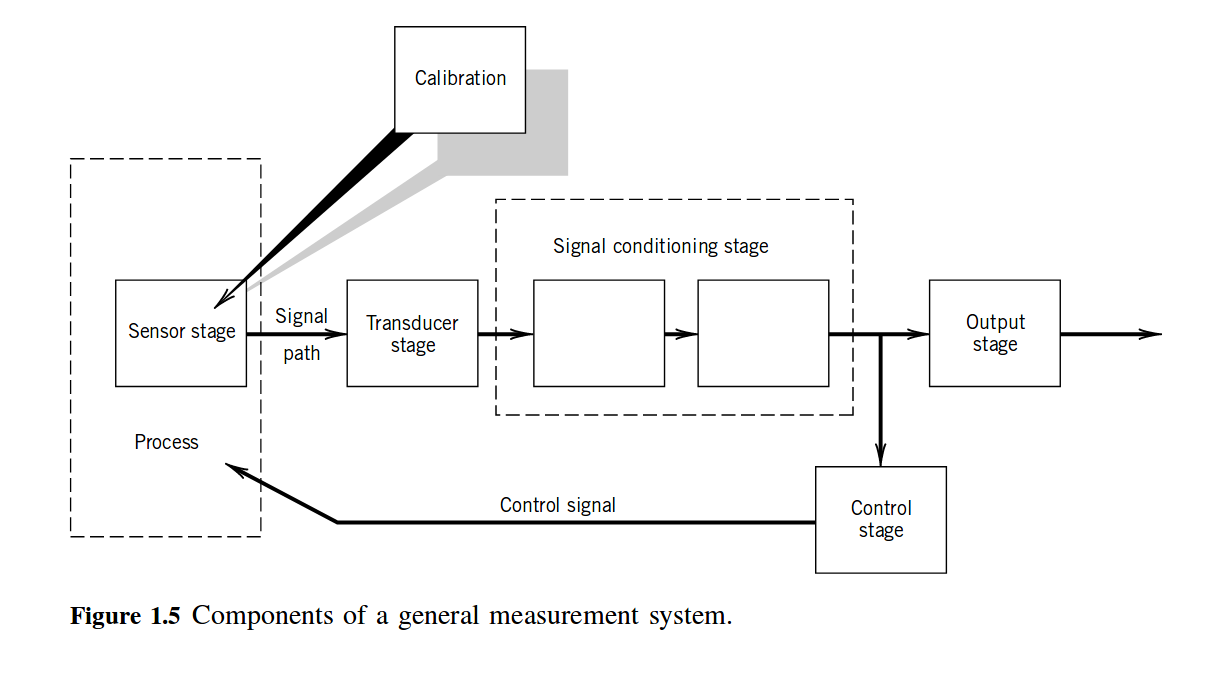
\includegraphics[scale=.3]{measurement_stages} \\
{\tiny Image: Theory and Design of Mech. Meas.}
\end{frame}

\begin{frame}
\frametitle{Sensor-Transducer Stage}
a {\PR sensor}, a physical element that employs some natural phenomenon... ...to sense the variable being measured
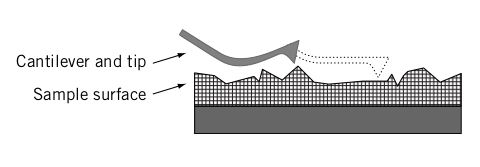
\includegraphics[scale=0.20]{sensor_stage.png}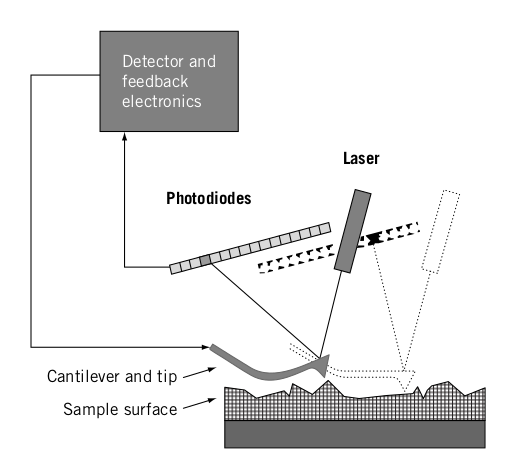
\includegraphics[scale=0.20]{sensor_transducer_stage}\\

A {\GR transducer} converts the sensed information into a detectable signal \\
{\tiny Text, Image: Theory and Design of Mech. Meas.}
\end{frame}

\frame{
\frametitle{Signal Conditioning Stage}

What is the the definition of {\BL signal}? \vspc

\begin{multicols}{2}
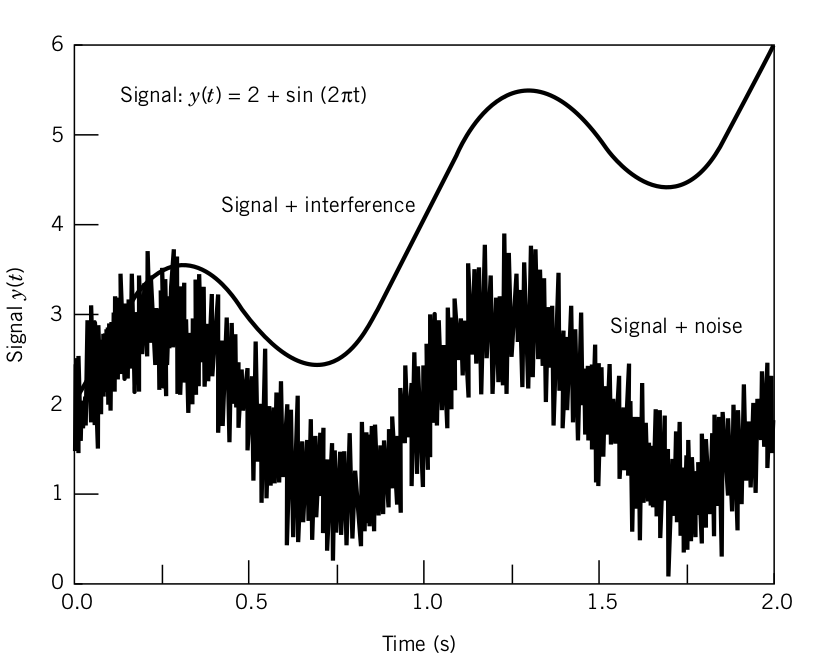
\includegraphics[scale=0.18]{signal_noise.png}

\begin{itemize}
\item Filtering
\item Amplification
\item Attenuation
\item Excitation 
\item Linearization
\item Electrical Isolation
\item Surge Protection
\end{itemize}

\end{multicols}

{\tiny Image: Theory and Design of Mech. Meas.}
}

\begin{frame}
\frametitle{Output Stage}
The {\BR output stage} indicates or records the value measured. This might be a simple readout
display, a marked scale, or even a recording device such as a computer disk drive.

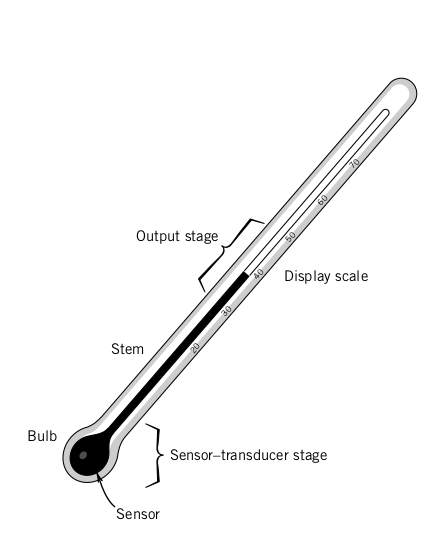
\includegraphics[scale=0.25]{bulb_thermometer.png} \hspace{10mm}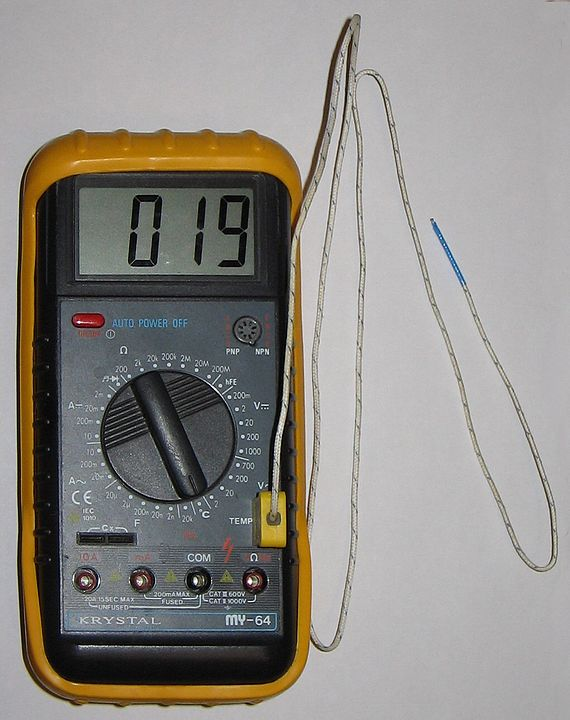
\includegraphics[scale=0.3]{thermocouple.jpg}

{\tiny Image: Theory and Design of Mech. Meas. \hspace{20mm} Image: \href{https://en.wikipedia.org/wiki/Thermocouple}{Wikipedia} }
\end{frame}

% Section 4
\section{\sectiontitleIV}

	\begin{frame}[label=sectionIV]
	\frametitle{\sectiontitleIV}

		\scriptsize
		\begin{multicols}{2}
			{\bf Activity:} Team Brainstorm

			{\bf Duration:} $\sim 10$ minutes

			{\bf Groups:} 2-3 members

			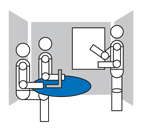
\includegraphics[scale=0.5]{Brainstorm_room.png}

			{\bf Topic:} Remote Probe Concept
			\begin{itemize}
				\item You are designing a remote probe to inspect an environment which can only be accessed from above. 
				\item The goal is to collect as much information as possible from the environment to prepare for a robotic maintinence task. 
	        \end{itemize}

	    \end{multicols}	

	    {\bf Requirements:}	
		\begin{itemize}
			\item Probe must enter environment through hole $\sim 100mm$ wide 
			\item Probe must exit through same hole leaving nothing behind
			\item The alllowable EFI and RFI is limited. No wifi communication is available \vspace{4mm}
		\end{itemize}

		{\bf Deliverable:} Submit a copy of your team brainstorming notes including text, images, and diagrams to the activity assignment on ilearn. Include names of all team members.

	\end{frame}

% Section 5
\section{\sectiontitleV}

\begin{frame}[label=sectionV]
\frametitle{\sectiontitleV}
\href{https://events-platform.asmeconferences.org/event/idetc-cie-2022/planning/UGxhbm5pbmdfOTcxMjI2}{IDETC2022-96785: Development of an Instrumented Rear Suspension to Measure the Tire Forces of a Race Car During Track Driving}\vspace{5mm}\\


\includegraphics[scale=0.125]{IDETC_technical_session.png}

\end{frame}

\begin{frame}[label=sectionV]
\frametitle{\sectiontitleV}

\href{https://events-platform.asmeconferences.org/event/idetc-cie-2022/planning/UGxhbm5pbmdfOTcxMzIx}{IDETC2022-91154: Photometric Stereo Enhanced Light Sectioning Measurement for Microtexture Road Profiling}\vspace{5mm}\\


\includegraphics[scale=0.125]{IDETC_technical_session.png}
 
\end{frame}

\begin{frame}[label=sectionV]
\frametitle{\sectiontitleV}
\href{https://events-platform.asmeconferences.org/event/idetc-cie-2022/planning/UGxhbm5pbmdfOTcxNDk4}{IDETC2022-90082: Automated Weld Path Generation Using Random Sample Consensus and Iterative Closest Point Workpiece Localization}\vspace{5mm}\\


\includegraphics[scale=0.125]{IDETC_technical_session.png}

\end{frame}

\end{document}





